\documentclass[letterpaper, 10 pt, conference]{ieeeconf}  % Comment this line out if you need a4paper

%\documentclass[a4paper, 10pt, conference]{ieeeconf}      % Use this line for a4 paper

\IEEEoverridecommandlockouts                              % This command is only needed if 
                                                          % you want to use the \thanks command

\overrideIEEEmargins                                      % Needed to meet printer requirements.




% The following packages can be found on http:\\www.ctan.org
\usepackage{graphics} % for pdf, bitmapped graphics files
\usepackage{epsfig} % for postscript graphics files
% \usepackage{times}
% \usepackage{newtxtext,newtxmath} % Times-like text and math fonts

\usepackage{mathptmx} % assumes new font selection scheme installed
\usepackage{times} % assumes new font selection scheme installed
\usepackage{amsmath} % assumes amsmath package installed
\usepackage{amssymb}  % assumes amsmath package installed
% \usepackage[utf8]{inputenc}

\usepackage{cite} % Use cite.sty for numerical citation management
\usepackage[bookmarks=true]{hyperref} % Use hyperref for other links
% \usepackage{hyperref} % Use hyperref for other links
% \usepackage{appendix}

\usepackage{tikz}
\usepackage{float}
\usepackage{svg}
% \usepackage{bm}
\usepackage{balance}

\tikzstyle{block} = [rectangle, minimum width=2cm, minimum height=1cm,text centered, draw=black]
\tikzstyle{block_1} = [rectangle, minimum width=2cm, minimum height=1cm,text centered, draw=black, fill=blue!5]
\tikzstyle{block_2} = [rectangle, minimum width=2cm, minimum height=1cm,text centered, draw=black, fill=red!5]
\tikzstyle{arrow} = [thick,->,>=stealth]
\tikzstyle{arrow_2} = [very thick,->,>=stealth]
\tikzstyle{arrow_3} = [thick,->,>=stealth,dashed]
\tikzstyle{pfr} = [cylinder, draw, minimum height=4cm, minimum width=1cm, shape aspect=1, shape border rotate=180]
\usetikzlibrary{shapes.geometric}


% Override the fake natbib command to allow cite.sty and hyperref to work together
\makeatletter
\let\NAT@parse\undefined
\makeatletter

\title{\LARGE \bf
Observer-based MPC of an Axial Dispersion Tubular Reactor:\\ Addressing Recycle Delays through Transport PDEs
}


\author{Behrad Moadeli and Stevan Dubljevic$^{1}$% <-this % stops a space
\thanks{$^{1}$Behrad Moadeli and Stevan Dubljevic are with the Department of Chemical and Materials Engineering,
University of Alberta, Edmonton, AB, Canada T6G 1H9
{\tt\small moadeli@ualberta.ca}, {\tt\small stevan.dubljevic@ualberta.ca}}%
\thanks{Funding provided by the Natural Sciences and Engineering Research Council of Canada—NSERC (RGPIN-2022-03486).}% <-this % stops a space
}


\begin{document}



\maketitle
\thispagestyle{empty}
\pagestyle{empty}


%%%%%%%%%%%%%%%%%%%%%%%%%%%%%%%%%%%%%%%%%%%%%%%%%%%%%%%%%%%%%%%%%%%%%%%%%%%%%%%%
\begin{abstract}

        The model predictive control of an axial dispersion tubular reactor equipped with a recycle stream is presented. The intrinsic time delay imposed by the recycle stream, an often overlooked aspect in chemical engineering process control studies, is modeled as a transport PDE, leading to a boundary-controlled system of coupled parabolic and hyperbolic PDEs under Danckwerts boundary conditions, suitable for this reactor type. Considering the digital nature of controllers, a discrete-time linear model predictive controller is designed to stabilize the system, coupled with a Luenberger state estimator to address the controller's limited access to the system's full state. The need for model reduction through spatial approximation is eliminated by following a late lumping approach, while utilizing Caley-Tustin time discretization method to preserve the continous-time system's characteristics. The controller's effectiveness is demonstrated through numerical simulations, showcasing its capability to stabilize an unstable system while adhering to input constraints, having access merely to output measurements.

\end{abstract}

\section{Introduction}

Many processes in the chemical and petrochemical sectors involve states that evolve over space and time, commonly represented by partial differential equations (PDEs) as distributed parameter systems (DPS) \cite{ray1981advanced}. 
The infinite-dimensional nature of DPSs presents specific challenges in control and estimation, making this a prominent area of research. Two main methods are often applied to control DPSs: \textit{Early Lumping} and \textit{Late Lumping}. 
Early Lumping reduces the system to a finite-dimensional approximation through spatial discretization early in the modeling stage, allowing for the application of standard control techniques \cite{davison1976robust}. 
However, this method can lead to inaccuracies due to mismatches between the reduced model and the original system dynamics \cite{moghadam2012infinite}. 
Late Lumping, by contrast, preserves the system's infinite-dimensional structure until the final stages of controller implementation, resulting in a control approach that is more complex but achieves greater fidelity to the original dynamics.

A range of studies in chemical engineering have applied the late lumping method to control infinite-dimensional systems, specifically targeting convection-reaction processes governed by first-order hyperbolic PDEs and diffusion-convection-reaction processes described by second-order parabolic PDEs. 
In \cite{christofides1996feedback}, the robust control of first-order hyperbolic PDEs is explored, demonstrating the stabilization of a plug flow reactor system using a distributed input. 
A boundary feedback stabilization approach using the backstepping method is presented in \cite{krstic2008backstepping} for a comparable system of first-order hyperbolic PDEs. 
The work in \cite{xu2016state} introduces a state feedback regulator design for a countercurrent heat exchanger system, providing another example of a chemical engineering DPS governed by first-order hyperbolic PDEs, distinct from tubular reaction systems. 
Highlighting the role of dispersion in axial dispersion tubular reactors, \cite{christofides1998robust} examines the robust control of diffusion-convection-reaction systems governed by second-order parabolic PDEs. 
In \cite{dubljevic2006predictive2}, a late-lumping approach is employed to develop a low-dimensional predictive controller for a diffusion-convection-reaction system, utilizing modal decomposition to capture the system's dominant modes. 
A similar method is applied in \cite{khatibi2021model} to design an observer-based model predictive controller (MPC) for an axial dispersion tubular reactor, accounting for the impact of recycle streams, a common feature in industrial chemical reactors. 
Different aspects of state reconstruction for DPSs are addressed in several works where the design of a discrete-time Luenberger observer is adressed for the class of DPSs, where no spatial discretization is required; a key feature of the late lumping approach  \cite{dochain2000state, dochain2001state, alonso2004optimal, ali2015review}.

In addition to dynamic systems distributed over space, dynamic systems that exhibit time delays are also classified as DPSs \cite{curtainbook}. 
In the field of control theory for infinite-dimensional systems, delay systems are either represented as delay differential equations (DDEs) or as transport PDEs, with the latter being advantageous in more complex scenarios, e.g. in the presence of spatial dynamics \cite{krstic2009book}. 
When it comes to chemical engineering applications of control theory, delays are often introduced as the result of input or output delays, while state delays are less frequently addressed in the literature; most probably since not many applications in this field can be described by state delays, in contrast with other domains of control theory, such as signal processing or mechanical systems. 
Input/output delays are generally handled by introducing a transportation lag block at either the input or output of the system, leading to a cascade PDE system \cite{Hiratsuka1969IEEE, mohammadi2012lq, Guilherme2019ACC}. 
In one of the few studies addressing state delays in this area, \cite{ozorio2019heat} investigates a delayed-state distributed parameter system where a full-state and output feedback regulator is designed for a heat exchanger system. 
Here, the state delay arises from the time taken for a stream to exit one pass of the heat exchanger and enter the next. 
Similarly, in \cite{qi2021output}, a tubular reactor system is considered, where state delay is introduced by the recycle delay in the system, without accounting for the diffusion term along the reactor. 
Even in \cite{khatibi2021model}, where a recycle stream is incorporated for a distributed diffusion-convection-reaction system, the recycle is assumed to be instantaneous—an assumption that creates a gap in the literature on diffusion-convection-reaction systems with recycle streams that impose a state delay.

In this work, an axial dispersion tubular reactor equipped with recycle is addressed as a diffusion-convection-reaction DPS. First, the reactor is modeled by a second order parabolic PDE, where the recycle stream poses a state delay, resulting in a first order hyperbolic transport PDE. 
Therefore, a system of coupled hyperbolic and parabolic PDEs is obtained to describe the infinite-dimensional model of the plant. 
The resolvent operator of the system is then obtained in an exact closed form, omitting the need for spatial discretization following the late lumping approach. 
The continous-time system is then discrtetized to enable the implementation of MPC as a digital controller. This is done using Caley-Tustin time discretization technique, i.e. a Crank-Nicolson type of discretization that preserves the conservative characteristics of the continuous system, mitigating the need for model reduction \cite{havu2007cayley, xu2017linear}. 
An infinite-dimensional Luenberger observer is also designed to reconstruct the states of the system, addressing the controller's limited access to system's full-state. 
As a result, through numerical simulations, the observer-based output feedback MPC is shown to successfully stabilize a system while adhering to input constraints, despite the original system being unstable.
\section{Continuous-time Model Representation}
Fig.~\ref{fig:reactor_scheme} illustrates a chemical process, i.e. a first-order irreversible reaction within an axial dispersion tubular reactor \cite{levenspiel1998chemical}. The reactor is equipped with a recycle mechanism, allowing a portion of the product stream to re-enter the reactor, increasing the conversion of the substrate.  Utilizing first-principle modeling through relevant mass balance relations on an infinitesimally thin disk element along the longitudinal axis of the reactor, the dynamics describing the concentration within the system results in a second-order parabolic PDE, a common class of equations used to characterize diffusion-convection-reaction systems \cite{jensen1982bifurcation}. 
\begin{figure}[!htbp] 
    \centering
    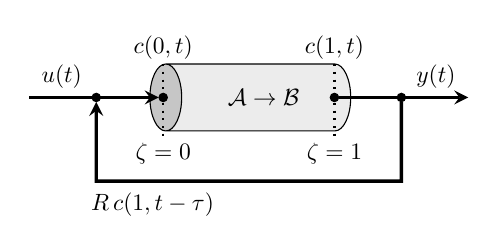
\begin{tikzpicture}[scale=0.85, transform shape]
        \node (pfr) [cylinder, draw, minimum height=3cm, minimum width=1cm, shape aspect=1, shape border rotate=180, cylinder uses custom fill, cylinder end fill=gray!45, cylinder body fill=gray!15] {$\mathcal{A} \rightarrow \mathcal{B}$};
        \node (pfr_inlet) [circle, left of=pfr, xshift=-0.5cm, fill=black, draw, inner sep=0pt, minimum size=0.25cm, scale=0.5] {};
        \node (pfr_outlet) [circle, at={(pfr.east)}, shift={(-0.25cm,0)}, fill=black, draw, inner sep=0pt, minimum size=0.25cm, scale=0.5] {};
        \node (recycle_right) [circle, right of=pfr_outlet, fill=black, draw, inner sep=0pt, minimum size=0.25cm, scale=0.5] {};
        \node (recycle_left) [circle, left of=pfr_inlet, fill=black, draw, inner sep=0pt, minimum size=0.25cm, scale=0.5] {};
        
        \draw[dotted, thick] ([yshift=0.5cm]pfr_inlet.center) -- node[at end, below, yshift=0.1cm] {$\zeta = 0$} ([yshift=-0.65cm]pfr_inlet.center);
        \draw[dotted, thick] ([yshift=0.5cm]pfr_outlet.center) -- node[at end, below, yshift=0.1cm] {$\zeta = 1$} ([yshift=-0.65cm]pfr_outlet.center);
        
        \node[below of=recycle_left, node distance=1.3cm, anchor=north west, xshift=-0.2cm] {$R \, c(1, t-\tau)$};
        \node[above of=pfr_inlet, node distance=0.75cm,] {$c(0, t)$};
        \node[above of=pfr_outlet, node distance=0.75cm,] {$c(1, t)$};
        
        \draw [arrow_2] (pfr_outlet) -- node[near end, above] {$y(t)$} ++(2,0);
        \draw [arrow_2] (pfr_inlet) ++(-2,0) coordinate(start) -- node[near start, above] {$u(t)$} (pfr_inlet);
        \draw [arrow_2] (recycle_right) -- ++(0,-1.25) -| (recycle_left);
        
    \end{tikzpicture}
    \caption{Axial tubular reactor with recycle stream.}
    \label{fig:reactor_scheme}
    % \pdfbookmark[2]{Figure: Reactor Scheme}{fig:reactor_scheme}
\end{figure}

In an attempt to make the model more realistic for common axial dispersion tubular reactors in chemical industry, Dankwerts boundary conditions are chosen as they are known to be suitable for this purpose by accounting for deviations from perfect mixing and piston flow, assuming negligible transport lags in connecting lines \cite{danckwerts1993continuous}. The delayed state resulting from the recycled portion of the flow, occurring $\tau$ seconds back in time, is applied at the inlet boundary condition. The governing equation along with the boundary conditions are given by \eqref{eq:PDE_original_model}.

\begin{equation} \label{eq:PDE_original_model}
    \begin{aligned}
        &\dot{c}(\zeta, t) = D \partial_{\zeta \zeta} c(\zeta, t) - v \partial_\zeta c(\zeta, t) + k_r c(\zeta, t) \\
        &\begin{cases}
            &D \partial_\zeta c(0, t) - v c(0, t) = -v \left[ R c(1, t-\tau) + (1-R) u(t) \right] \\
            &\partial_\zeta c(1, t) = 0 \\
            &y(t) = c(1, t)
        \end{cases}
    \end{aligned}
\end{equation}

Here, $c(\zeta, t)$ is the concentration along the reactor, representing the state of the system. The physical parameters $D$, $v$, $k_r$, $R$, and $\tau$ represent the diffusion coefficient, flow velocity along the reactor, reaction constant, recycle ratio, and residence time of the recycle flow, respectively. The coordinate system in space and time is represented by $\zeta$ and $t$, where $\zeta \in [0, 1]$ and $t \in [0, \infty)$.

An interesting approach to address delays where the problem involves other forms of PDEs is to reformulate the problem such that the notion of delay is replaced with an alternative transport PDE \cite{krstic2009book}. 
Therefore, the state variable $c(\zeta,t)$ is replaced with a new state variable $\underline{x}(\zeta, t) \equiv [x_1(\zeta, t), x_2(\zeta, t)]^T$ as a vector of functions, where $x_1(\zeta, t)$ represents the concentration within the reactor—analogous to $c(\zeta,t)$—and $x_2(\zeta, t)$ is the new state variable for the concentration along the recycle stream. The delay is thus modeled as a pure transport process rather than being present in the argument of the state at the boundary—i.e. $c(1,t-\tau)$— making all state variables expressed explicitly at a specific time instance $t$, resulting in the standard state-space form for an infinite-dimensional linear time-invariant (LTI) system given in \eqref{eq:state_space}.
\begin{equation} \label{eq:state_space}
    \begin{aligned}
        \dot{\underline{x}}(\zeta, t) &= \mathfrak{A} \underline{x}(\zeta, t) + \mathfrak{B} u(t) \\
        y(t) &= \mathfrak{C} \underline{x}(\zeta, t)
    \end{aligned}
\end{equation}
Here, $\mathfrak{A}$ is a linear operator $\mathcal{L}(X)$ acting on a Hilbert space $X: L^2[0,1] \times L^2[0,1]$ and $\underline{x}(\zeta,t)$, as defined previously, is the vector of functions describing the states of the system. The operators ($\mathfrak{A}$, $\mathfrak{B}$, $\mathfrak{C}$, and $\mathfrak{D}$) are defined in \eqref{eq:operator_A} for the infinite-dimensional LTI system.

\begin{equation} \label{eq:operator_A}
    \begin{aligned}
        \mathfrak{A} &\equiv
        \begin{bmatrix}
            D \partial_{\zeta \zeta} - v \partial_\zeta + k_r & 0 \\
            0 & \frac{1}{\tau} \partial_\zeta
        \end{bmatrix} \hspace{0.4em}
        \mathfrak{B} \equiv
        \begin{bmatrix}
            \delta(\zeta) \\
            0
        \end{bmatrix} \cdot (1-R) v \\
        \mathfrak{C} &\equiv
        \begin{bmatrix}
            \delta(\zeta-1) &
            \hspace{3.7em} 0 \hspace{0.6em}
        \end{bmatrix} \hspace{0.42em}
        \mathfrak{D} = 0
        % \mathcal{D}(\mathfrak{C}) &= \mathcal{D}(\mathfrak{A})
    \end{aligned}
\end{equation}
with $\delta(\zeta)$ being dirac delta function. The system's spectrum can now be obtained by solving the eigenvalue problem for the system generator $\mathfrak{A}$. To do this, the characteristics equation of the system needs to be obtained by solving the equation $det(\mathfrak{A}-\lambda_i~I)~=~0$ for $\lambda_i$, where $\lambda_i \in \mathbb{C}$ is the $i^{\text{th}}$ eigenvalue of the system and $I$ is the identity operator. Attempts to analytically solve this equation will fail; therefore, it is solved numerically given the parameters in Table~\ref{tab:pars}. The eigenvalue distribution is given in Figure~\ref{fig:eigval_dist} in the complex plane. This suggests that the open-loop system is unstable, as there are eigenvalues with positive real parts.

\begin{figure}[!htbp]
    \centering
    \includesvg[inkscapelatex=false, height=0.25\textwidth, keepaspectratio]{Figures/eig_val_dist_R_0.3.svg}
    \caption{Eigenvalues of operator $\mathfrak{A}$.}
    \label{fig:eigval_dist}
\end{figure}

\begin{table}[ht]
    \centering
    \caption{Physical Parameters for the System}
    \label{tab:pars}
    \begin{tabular}{|c|c|c|c|}
    \hline
    \textbf{Parameter}        & \textbf{Symbol} & \textbf{Value}     & \textbf{Unit}    \\ \hline
    Diffusivity               & $D$             & $2\times10^{-5}$   & ${m^2}/{s}$      \\ \hline
    Velocity                  & $v$             & $0.01$   & ${m}/{s}$        \\ \hline
    Reaction Constant         & $k_r$           & $1.5$              & $s^{-1}$         \\ \hline
    Recycle Residence Time    & $\tau$          & $80$               & $s$              \\ \hline
    Recycle Ratio             & $R$             & $0.3$              & $-$              \\ \hline
    \end{tabular}
\end{table}

The exact closed-form representation for the resolvent operator is derived in Appendix \ref{app:resolvent}. Since the system is not self-adjoint, the adjoint system operators $\mathfrak{A}^*$ and $\mathfrak{B}^*$ as well as the resolvent operator for the adjoint system must be obtained in the same manner as the original system. However, this is not included in the manuscript to avoid redundancy.
\input{sections/03_discrete}
\section{Observer Design}

One important issue of DPSs is the limitted access to the states of the infinite-dimensional system as the state is distributed over the entire domain and performing infinite measurements is never feasible. Therefore, an observer is required to estimate the states of the system based on the available measurements. To address this issue, a Luenberger observer is designed to reconstruct the states of the system based on the output measurements. First, the consinuous-time observer design is considered; followed by the design of the discrete-time observer.

\subsection{Continuous-Time Observer Design}

For the purpose of state recunstruction of a diffusion-convection-reaction system, where the feedforward term $\mathfrak{D}$ is generally absent, the continuous-time observer dynamics are given by \eqref{eq:observer_continuous}.

\begin{equation} \label{eq:observer_continuous}
    \begin{aligned}
        \dot{\hat{x}}(\zeta, t) &= \mathfrak{A} \hat{x}(\zeta, t) + \mathfrak{B} u(t) + \mathfrak{L}_c [y(t) - \hat{y}(t)] \\
        \hat{y}(t) &= \mathfrak{C} \hat{x}(\zeta, t)
    \end{aligned}
\end{equation}

where $\hat{x}(\zeta, t)$ is the reconstructed state of the original system and $\mathfrak{L}_c$ is the continous-time observer gain. By subtracting the observer dynamics from the original system dynamics, the error dynamics $e(\zeta,t$) are obtained as shown in \eqref{eq:observer_error_continuous}.

\begin{equation} \label{eq:observer_error_continuous}
    \begin{aligned}
        \dot{e}(\zeta, t) &= (\mathfrak{A} - \mathfrak{L}_c \mathfrak{C}) e(\zeta, t) = \mathfrak{A}_o e(\zeta,t) \\
    \end{aligned}
\end{equation}

The goal is to design the observer gain $\mathfrak{L}_c$ such that the error dynamics are exponentially stable, i.e. $\max\{\operatorname{Re}(\lambda_{o})\}~<~0$ where $\lambda_{o}$ are the eigenvalues of the error dynamics matrix $\mathfrak{A}_o$. In Fig.~\ref{fig:L_vs_lambda}, three different forms of the observer gain are considered as spatial functions, with their effect on $\max\{\operatorname{Re}(\lambda_{o})\}$.

\begin{figure}[!htbp]
    \centering
    \includesvg[inkscapelatex=false, width=0.42\textwidth, keepaspectratio]{figures/obs_lambda.svg}
    \caption{Eigenvalues of operator $\mathfrak{A}$.}
    \label{fig:L_vs_lambda}
\end{figure}


\subsection{Discrete-Time Observer Design}


\section{Model Predictive Controller Design}

In this section, the observer-based MPC shown in Fig.~\ref{fig:block_diagram} is developed with the goal of stabilizing the given unstable infinite-dimensional system within an optimal framework, relying solely on output measurements while satisfying input constraints. 
An infinite-time open-loop objective function sets the foundation of the controller design in the discrete-time setting at each sampling instant $k$, which consists of a weighted sum of state deviations and actuation costs for all future time instances, subject to the system dynamics and input constraints, as shown in \eqref{eq:MPC_inf_time}.

\begin{figure}[!htbp]
    \centering
    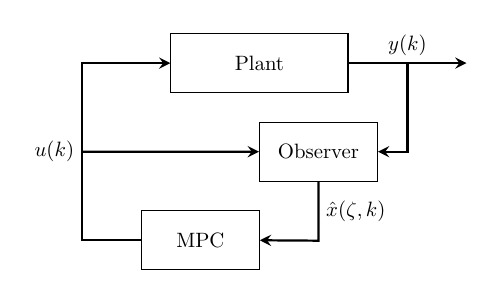
\begin{tikzpicture}[node distance=2cm, scale=0.75, transform shape]
        \node (plant) [block, minimum width=3cm] {Plant};
        \node (regulator) [block, below of=plant, xshift=-1cm, yshift=-1cm] {MPC};
        \node (observer) [block, below of=plant, xshift=1cm, yshift=0.5cm] {Observer};
        \draw [arrow] (plant.east) -- node[midway, above] {$y(k)$} ++(2,0);
        \draw [arrow] (plant.east) ++(1,0) |- (observer.east);
        \draw [arrow] (observer.south) -- ++(0,-1) node[midway, right] {$\hat{{x}}(\zeta,k)$} -- (regulator.east);    
        \draw [arrow] (regulator.west) -- ++(-1,0) |- (plant.west);
        \draw [arrow] (regulator.west) ++(-1,1.5) coordinate(start) -- node[near start, left, xshift=-0.75cm] {$u(k)$} (observer.west);
    \end{tikzpicture}
    \caption{Block diagram representation of the observer-based MPC.}
    \label{fig:block_diagram}
\end{figure}

\begin{equation} \label{eq:MPC_inf_time}
    \begin{aligned}
        \min_{U} \quad \sum_{l=0}^{\infty} &\langle \underline{\hat{x}}(\zeta, k+l | k), \mathfrak{Q} \underline{\hat{x}}(\zeta, k+l | k) \rangle \\
        + &\langle u(k+l+1 | k), \mathfrak{F} u(k+l+1|k) \rangle \\
        \, \\
        \text{s.t.} \quad &\underline{\hat{x}}(\zeta, k+l | k) = \mathfrak{A}_d \underline{\hat{x}}(\zeta, k+l-1 | k) + \mathfrak{B}_d u(k+l | k) \\
        &u^{min} \leq u(k+l | k) \leq u^{max}
    \end{aligned}
\end{equation}

where $\mathfrak{Q}$ and $\mathfrak{F}$ are positive definite operators of appropriate dimensions, responsible for penalizing state deviations and actuation costs, respectively. The notation $(k+l|k)$ indicates the future time states or input instance $k+l$ obtained at time $k$. The infinite-time optimization problem may be reduced to a finite-time setup by assigning zero-input beyond a certain control horizon $N$, resulting in the optimization problem in \eqref{eq:MPC_finite_time}.

\begin{equation} \label{eq:MPC_finite_time}
    \begin{aligned}
        \min_{U} \quad \sum_{l=0}^{N-1} &\langle \underline{\hat{x}}(\zeta, k+l | k), \mathfrak{Q} \underline{\hat{x}}(\zeta, k+l | k) \rangle \\
        + &\langle u(k+l+1 | k), \mathfrak{F} u(k+l+1|k) \rangle \\
        + &\langle \underline{\hat{x}}(\zeta, k+N | k), \mathfrak{P} \underline{\hat{x}}(\zeta, k+N | k) \rangle \\
        \, \\
        \text{s.t.} \quad &\underline{\hat{x}}(\zeta, k+l | k) = \mathfrak{A}_d \underline{\hat{x}}(\zeta, k+l-1 | k) + \mathfrak{B}_d u(k+l | k) \\
        &u^{min} \leq u(k+l | k) \leq u^{max} \\
        & \langle \underline{\hat{x}}(\zeta, k+N | k), \underline{\phi_u}(\zeta) \rangle = 0
    \end{aligned}
\end{equation}

Obtained as the solution to the discrete-time Lyapunov equation, $\mathfrak{P}$ is the terminal cost operator as shown in \eqref{eq:terminal_cost}; which can be proven to be positive definite only if the terminal state $\underline{\hat{x}}(\zeta, k+N | k)$ is in a stable subspace. Therefore, an equality constraint is introduced to guarantee that the resulting quadratic optimization problem is convex. The terminal constraint is enforced by setting the projection of the terminal state onto the unstable subspace of the system to zero \cite{curtainbook, xu2017linear, khatibi2021model}. Here, $\underline{\phi_u}(\zeta)$ is the set of unstable eigenfunctions of the system, for all eigenvalues where $\operatorname{Re}(\lambda_u) \geq 0$.

\begin{equation} \label{eq:terminal_cost}
    \mathfrak{P} (\cdot) = \sum_{m=0}^{\infty} \sum_{n=0}^{\infty} 
    -\frac{
        \langle \underline{\phi_m} , \mathfrak{Q} \underline{\psi_n} \rangle
    }{
        \lambda_m + \overline{\lambda_n}
    }
    \langle (\cdot) , \underline{\psi_n} \rangle \phi_m
\end{equation}

One may further process the optimization problem in \eqref{eq:MPC_finite_time} to obtain a standard format for quadratic programming (QP) solvers by substituting the future states in terms of the current state and the sequence of future inputs using system dynamics expression. The resulting QP problem is given in \eqref{eq:MPC_QP}. The optimal input sequence $U$ is then obtained by solving the QP problem at each sampling instant $k$. To implement a receding horizon control strategy, only the first input of the optimal sequence $u(k+1|k)$ is applied to the system, and the optimization problem is solved again at the next sampling instant $k+1$.

\begin{equation} \label{eq:MPC_QP}
    \begin{aligned}
        \min_{U} &J = U^T \langle I,H \rangle U + 2U^T \langle I, P \underline{\hat{x}}(\zeta, k|k) \rangle \\
        \text{s.t.} &\qquad U^{min} \leq U \leq U^{max} \\
        &\qquad T_u \underline{\hat{x}}(\zeta, k|k) + S_u U = 0
        \, \\
        \text{with } &H = \\
        &\hspace{-3.5em }\begin{bmatrix}
            \mathfrak{B}_d^* \mathfrak{P} \mathfrak{B}_d + \mathfrak{F} & \mathfrak{B}_d^* \mathfrak{A}_d^* \mathfrak{P} \mathfrak{B}_d & \cdots &  \mathfrak{B}_d^* {\mathfrak{A}_d^*}^{N-1} \mathfrak{P} \mathfrak{B}_d \\
            \mathfrak{B}_d^* \mathfrak{P} \mathfrak{A}_d \mathfrak{B}_d & \mathfrak{B}_d^* \mathfrak{P} \mathfrak{B}_d + \mathfrak{F} & \cdots & \mathfrak{B}_d^* {\mathfrak{A}_d^*}^{N-2} \mathfrak{P} \mathfrak{B}_d \\
            \vdots & \vdots & \ddots & \vdots \\
            \mathfrak{B}_d^* \mathfrak{P} {\mathfrak{A}_d}^{N-1} \mathfrak{B}_d & \mathfrak{B}_d^* \mathfrak{P} {\mathfrak{A}_d}^{N-2} \mathfrak{B}_d & \cdots & \mathfrak{B}_d^* \mathfrak{P} \mathfrak{B}_d + \mathfrak{F}
        \end{bmatrix} \\
        P = &\begin{bmatrix}
            \mathfrak{B}_d^* \mathfrak{P} {\mathfrak{A}_d} &
            \mathfrak{B}_d^* \mathfrak{P} {\mathfrak{A}_d}^{2}  &
            \hdots &
            \mathfrak{B}_d^* \mathfrak{P} {\mathfrak{A}_d}^{N} 
        \end{bmatrix}^T \\
        T_u (\cdot) = &\begin{bmatrix}
            \langle {\mathfrak{A}_d}^{N} (\cdot), \underline{\phi_u} \rangle
        \end{bmatrix} \\
        S_u = &\begin{bmatrix}
            \langle {\mathfrak{A}_d}^{N-1} \mathfrak{B}_d, \underline{\phi_u} \rangle & 
            \langle {\mathfrak{A}_d}^{N-2} \mathfrak{B}_d, \underline{\phi_u} \rangle &
            \hdots &
            \langle \mathfrak{B}_d, \underline{\phi_u} \rangle
        \end{bmatrix} \\
        U = &\begin{bmatrix}
            u(k+1|k) & u(k+2|k) & \hdots & u(k+N|k)
        \end{bmatrix}^T
    \end{aligned}
\end{equation}
\input{sections/06_results}
% \input{sections/07_conclusion}
\section*{Appendix}

\subsection{Resolvent Operator of the Original System}

\textbf{I have made enough space to include this here}

\subsection{Resolvent Operator of the Adjoint System}

% \section*{Acknowledgment}

\textbf{Do we need it?}
\textbf{Should I include Guilherme as an author?}


% Include the bibliography
% \addtolength{\textheight}{-15cm}
\balance
\bibliographystyle{IEEEtran}
\bibliography{./IEEEabrv,./references}  % Include both abbreviation and reference files



\end{document}
